% Beamer template
% Author: Ozgur Taylan TURAN
% Delft University of Technology

\documentclass[aspectratio=169]{beamer}
% PACKAGES
\usepackage[english]{babel}
\usepackage{graphicx}
\usepackage{animate}
%\usepackage{calc}
\usepackage{calligra}
\usepackage[absolute,overlay]{textpos}
\usepackage[T1]{fontenc}
%\usefonttheme{serif}
\usefonttheme{professionalfonts}
\usepackage{amsmath}
\usepackage{palatino}
\usepackage{mathpazo}
\usepackage{graphicx}
%\usepackage{subfig}
\usepackage{tikz}
\usetikzlibrary{shapes,arrows}
\usepackage{xcolor}
\usepackage[T1]{fontenc}
%\usefonttheme{serif}
%\usepackage{titling}
\usepackage{graphicx}
%\usepackage{subfig}
%\usepackage{tikz}
%\usetikzlibrary{shapes,arrows}
\usepackage{mathtools}
\usepackage{cancel}
% CUSTOM PACKAGES
\usepackage{/home/taylanot/texmf/tex/beamerthemetot}
\input{/home/taylanot/texmf/presentation/tune.tex}

 % COVER PAGE INFO   
\newcommand{\mytitle}{\color{White}\huge{\textbf{PR Lab Talk \#4}}}
\newcommand{\myjokesubtitle}{\color{Pink}\Large{\textbf{How to get a divorce with your supervisor?}}}
\newcommand{\mysubtitle}{\color{Pink}\Large{\textbf{What makes a good paper?}}}
\newcommand{\myauthor}{\color{White}\textcalligra{\LARGE Ozgur Taylan Turan}}
\newcommand{\authorlabel}{\small O.T. Turan}
\author{\authorlabel}

\setlength\bibitemsep{0.3cm} % space between entries in the reference list
\renewcommand{\bibfont}{\normalfont\scriptsize}
\renewcommand{\cite}[1]{\footnote<.->[frame]{\fullcite{#1}}}
\setbeamertemplate{bibliography item}{}
\bibliography{../../../../references/LabTalk.bib}


\begin{document}
% COVER PAGE
{
\def\beamer@entrycode{\vspace*{-\headheight}}
\setbeamertemplate{frametitle}[default][center]
\setbeamertemplate{navigation symbols}{}
\usebackgroundtemplate{
\includegraphics[width=\paperwidth,height=\paperheight]{cover/coverart.pdf}}

\begin{frame}[plain] 

\begin{minipage}{\textwidth}
	\centering{\mytitle} \\
	%\vspace{1cm}
	%\centering{\mysubtitle} \\
	\vspace{1cm}
	\centering{\color{White}November 15, 2021} \\
	\vspace{1cm}
	\centering{\myauthor}\\
\end{minipage}
\end{frame}
}


\begin{frame}
	\centering
	\myjokesubtitle
\end{frame}

\begin{frame}
	\centering
	\mysubtitle
\end{frame}

\begin{frame}{What makes a paper good?}
\begin{minipage}{0.25\textwidth}
  \begin{itemize}
    \item Attractive title?
    \item Cool figures?
    \item Proper writing?
    \item Outstanding results?
  \end{itemize}
\end{minipage}%
\begin{minipage}{0.75\textwidth}
  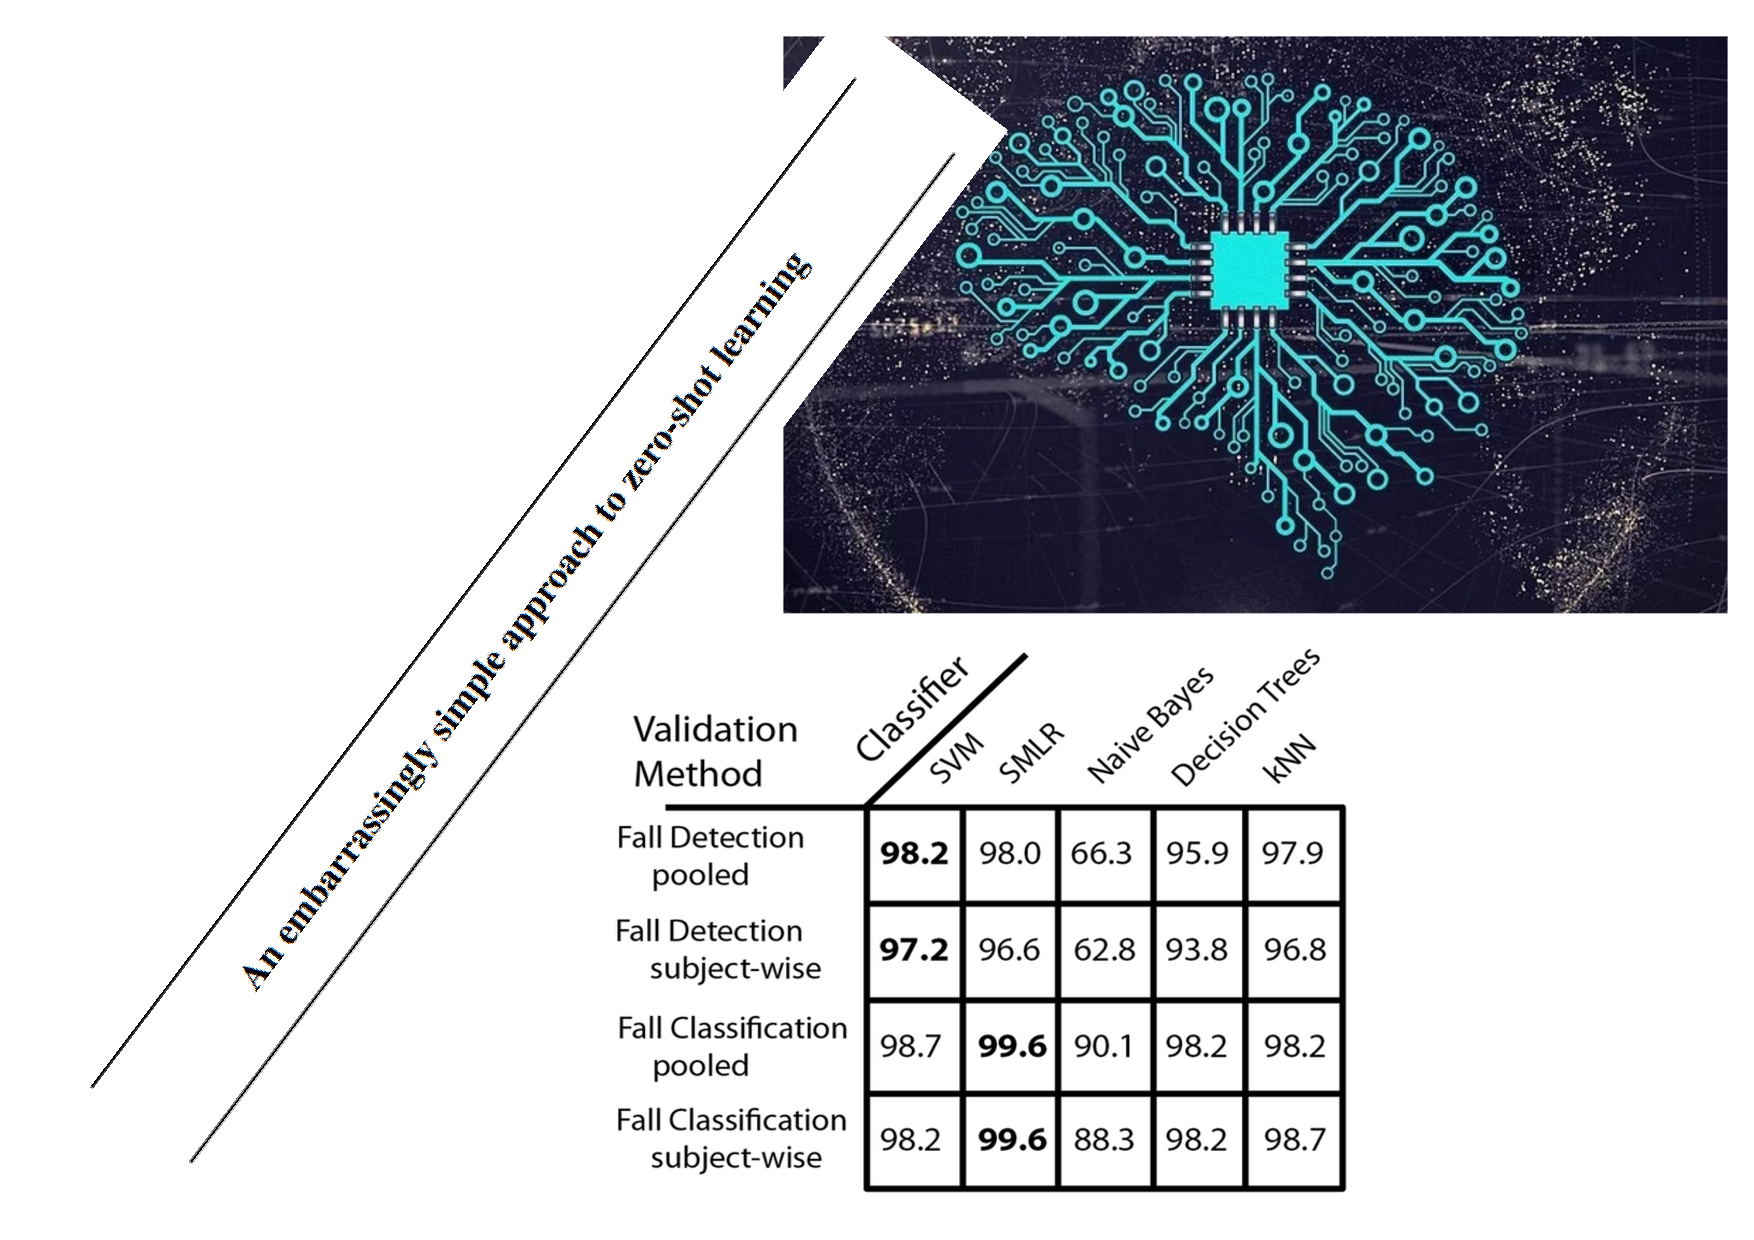
\includegraphics[width=0.9\textwidth]{Figures/collect.pdf}
\end{minipage}
\end{frame}

\begin{frame}{A paper}
  \begin{itemize}
    \item Main aim is to convey a message, right?
    \item In essence, tries to answer a question(s)! (Research Question?)
  \end{itemize}
  \centering
  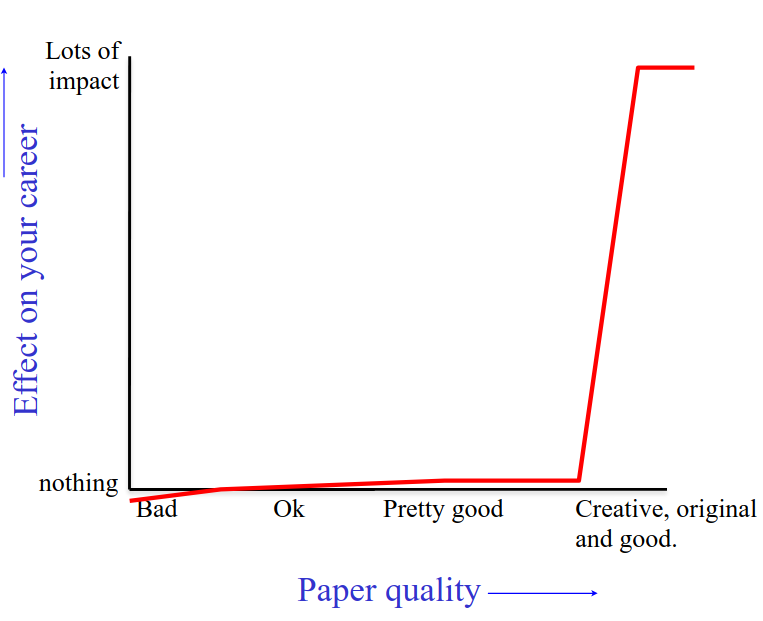
\includegraphics[width=0.4\textwidth]{Figures/quality.png}

    [According to Jan's suggested link]
\end{frame} 

\begin{frame}{RQ}
\begin{minipage}{0.5\textwidth}
  \begin{itemize}
    \item MSc student: "How do you formulate a research question? They did not teach this to us!"
    \item Then, how do we learn how to do it?
  \end{itemize}
\end{minipage}%

\end{frame} 

\begin{frame}{Some Info - RQ in papers}
  \begin{itemize}
    \item Research purpose vs Research Question
  \end{itemize}
  \centering
  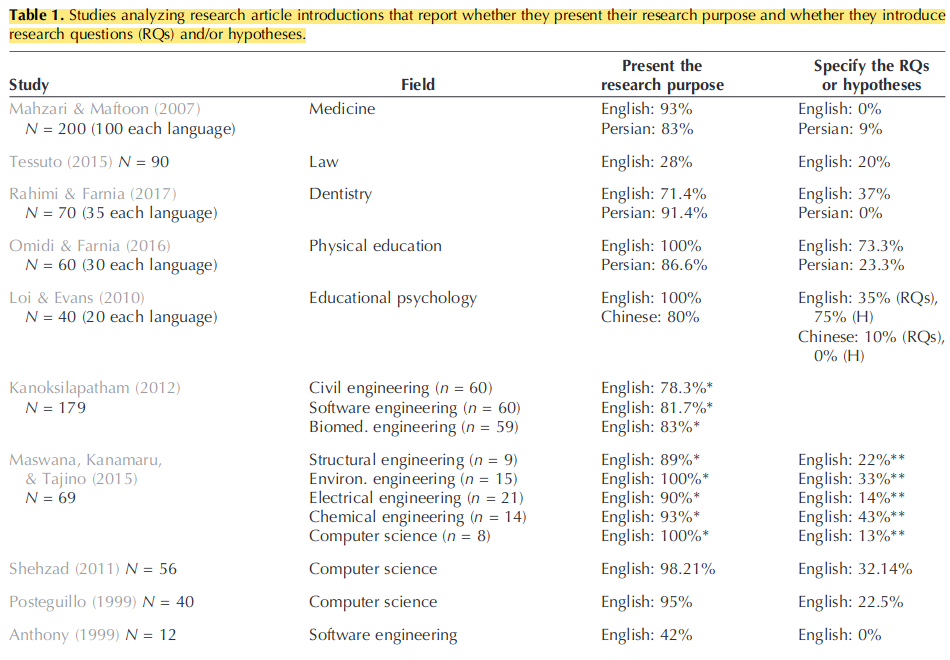
\includegraphics[width=0.45\textwidth]{Figures/pvq.png}\cite{thelwall2020}
\end{frame} 

\begin{frame}{Some Info - How to formulate?}
  \begin{itemize}
    \item Stephan's discussion last week?
  \end{itemize}
  \centering
  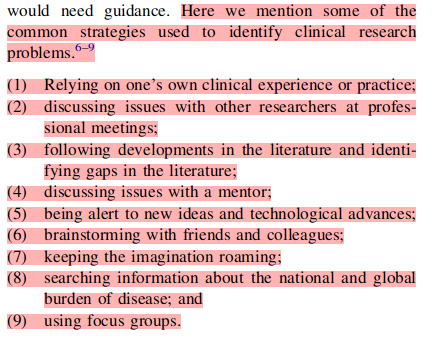
\includegraphics[width=0.45\textwidth]{Figures/how.png}\cite{thabane2009}
\end{frame}

\begin{frame}{Points of Discussion...}
  \begin{itemize}
    \item How did you learn to formulate a Research Question?
    \item Do you use systematic way for formulating a Research Question?
    \item Do you explicitly mention you research questions?
    \item Do senior researches nail it every time?
    \item Is it related to the environment you are in?
  \end{itemize}
\end{frame}

\end{document}
